\section{抽样与方差控制}
\label{sec:opt-sto-variance}

上一节的误差界里，噪声通过$\sigma_\star^2$或$\sigma^2$进入，并在常数步长下形成平台。本节保持目标不变，只改变读数的取得方式，看能否用额外的读取或存储换来更小的方向噪声。四种做法依次是：按不同概率抽取各项、一次读取多项、在快照点用完整梯度纠偏，以及为每一项保存一份旧梯度。前两种只把噪声按比例缩小，后两种在有限和上能让噪声随迭代趋于零。

\subsection{非均匀抽样与重加权}
\label{sec:opt-sto-importance}

\paragraph{反比权重}
各项的“分量”常常不同：最小二乘中，范数大的行梯度也大。很自然的想法是更常抽重要的项。设目标为$f(\bm x)=\frac1n\sum_i\ell_i(\bm x)+r(\bm x)$，$r$是确定的正则项，以概率$p_i>0$（$\sum_ip_i=1$）抽取下标$I$。要让读数仍条件无偏，抽到的项必须按抽样概率的倒数加权：
\begin{equation}
\label{eq:opt-sto-importance}
  \bm g=\frac{\nabla\ell_I(\bm x)}{np_I}+\nabla r(\bm x),\qquad
  \mathbb E_t[\bm g]=\sum_{i=1}^np_i\frac{\nabla\ell_i(\bm x)}{np_i}+\nabla r(\bm x)=\nabla f(\bm x).
\end{equation}
被抽得多的项每次贡献得少，被抽得少的项每次贡献得多，平均下来各项权重仍是$1/n$。这种做法是\term{重要性采样}（importance sampling）在优化中的用法。正则梯度$\nabla r(\bm x)$是确定量，不随抽样变化，每次读数只加一次，不参与重加权。

\paragraph{两项例：偏差与二阶矩}
取$n=2$，在某点$\nabla\ell_1=2$、$\nabla\ell_2=-1$，$r=0$，真梯度为$1/2$。按$p=(3/4,1/4)$抽样但不重加权，读数的平均是$\tfrac34\cdot2+\tfrac14\cdot(-1)=5/4$，偏差$3/4$。重加权后两种读数变为$2/(2\cdot\tfrac34)=4/3$与$-1/(2\cdot\tfrac14)=-2$，平均回到$1/2$。

无偏之后再看二阶矩。由式~\eqref{eq:opt-sto-importance}，
\begin{equation}
\label{eq:opt-sto-importance-moment}
  \mathbb E_t\Bigl\lVert\frac{\nabla\ell_I(\bm x)}{np_I}\Bigr\rVert_2^2=\frac1{n^2}\sum_{i=1}^n\frac{\lVert\nabla\ell_i(\bm x)\rVert_2^2}{p_i}
  \geq\Bigl(\frac1n\sum_{i=1}^n\lVert\nabla\ell_i(\bm x)\rVert_2\Bigr)^2 ,
\end{equation}
不等式由Cauchy--Schwarz不等式$\bigl(\sum_i\lVert\nabla\ell_i\rVert_2\bigr)^2=\bigl(\sum_i\sqrt{p_i}\cdot\lVert\nabla\ell_i\rVert_2/\sqrt{p_i}\bigr)^2\leq\sum_ip_i\cdot\sum_i\lVert\nabla\ell_i\rVert_2^2/p_i$得到，等号在$p_i\propto\lVert\nabla\ell_i(\bm x)\rVert_2$时成立。两项例中，均匀抽样的二阶矩为$(4+1)/2=5/2$，$p=(3/4,1/4)$时为$\tfrac34\cdot\tfrac{16}9+\tfrac14\cdot4=7/3$，最优的$p=(2/3,1/3)$给出$9/4$；而反过来取$p=(1/4,3/4)$，读数变为$4$与$-2/3$，二阶矩升到$13/3$。抽样概率很小的项一旦被抽中，读数会被放大$1/(np_i)$倍，选错概率比均匀抽样更糟。

\paragraph{按光滑常数抽样}
最优概率依赖于当前点的梯度，每步重算要读全部项，失去了抽样的意义。实用的替代是按光滑常数抽样：若$\ell_i$凸且$L_i$光滑，$r$凸且$\lambda$光滑，令$\phi_i=\ell_i/(np_i)+r$，则$f=\sum_ip_i\phi_i$，读数恰为$\nabla\phi_I(\bm x)$，$\phi_i$凸且$\bigl(L_i/(np_i)+\lambda\bigr)$光滑。在引理~\ref{lem:opt-sto-distance}的证明中把均匀平均换成$p$加权平均，结论不变，只需把$L_{\max}$换成$\max_iL_i/(np_i)+\lambda$、把$\sigma_\star^2$换成$\sigma_{\star,p}^2=\sum_ip_i\lVert\nabla\phi_i(\bm x^\star)\rVert_2^2$。取$p_i=L_i/\sum_jL_j$时，前者变为平均光滑常数$\bar L+\lambda$，$\bar L=\frac1n\sum_iL_i$。少数几项特别陡时，$\bar L$远小于$\max_iL_i$，允许的步长和定理~\ref{thm:opt-sto-decreasing}中的$t_0$都随之改善\scite{needell2016stochastic}。代价是$\sigma_{\star,p}^2$可能变大：最小点处梯度大的项未必是光滑常数大的项。

图~\ref{fig:opt-sto-importance}展示这一取舍。数据中前$4$行被放大$6$倍，$L_{\max}\approx80.6$，而平均光滑常数只有约$5.64$。按$p_i\propto\lVert\bm a_i\rVert_2^2$抽样并重加权后，$t_0$从约$458$降到约$32$，误差早早开始下降；但最小点处的噪声从$\sigma_\star^2\approx0.645$升到$\sigma_{\star,p}^2\approx1.12$，到$3000$步时均匀抽样反而略低。不重加权的运行则收敛到另一个点，误差停在红色虚线处，那是把加权平均$\sum_ip_i\nabla\ell_i$当作梯度时的驻点。

\begin{figure*}[!htbp]
  \centering
  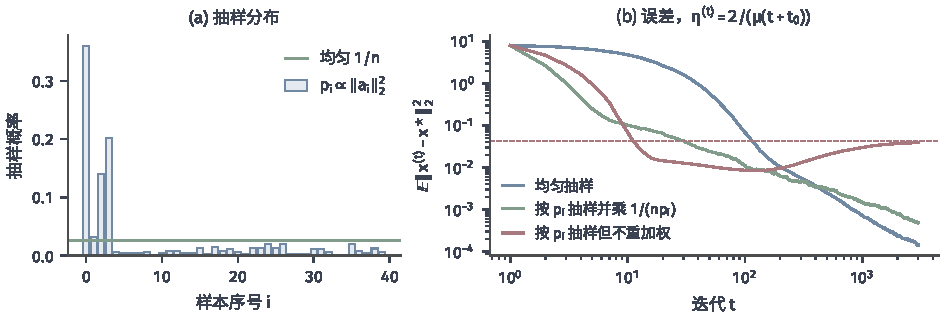
\includegraphics[width=160mm]{figures/03-optimization-evolution-and-signals/01-optimization/matplotlib/c6-importance-sampling/figure.pdf}
  \caption{非均匀抽样。$n=40$、$d=2$的岭回归最小二乘，前$4$行放大$6$倍。(a) 按$p_i\propto\lVert\bm a_i\rVert_2^2$的抽样概率与均匀概率$1/n$。(b) $300$次运行的平均平方距离，双对数坐标，三条曲线都用递减步长$2/(\mu(t+t_0))$：蓝线为均匀抽样，$t_0=4L_{\max}/\mu\approx458$；绿线按$p_i$抽样并乘$1/(np_i)$，$t_0=4(\bar L+\lambda)/\mu\approx32$；红线按$p_i$抽样但不重加权，步长同蓝线，它收敛到有偏的驻点，红色虚线标出该点到$\bm x^\star$的平方距离。}
  \label{fig:opt-sto-importance}
\end{figure*}

\paragraph{抽样本身的成本}
非均匀抽样还要算上维护分布的成本。概率固定时，用别名表可以$O(n)$预处理、$O(1)$抽样；概率随迭代变化时，常用树结构在$O(\log n)$时间内更新与抽样。若概率要靠估计各项的当前梯度来设定，估计所需的读取也要计入。比较抽样策略时，应在同样的读取与计算预算下比较误差，而不是只比较迭代次数。

\subsection{小批量与梯度累积}
\label{sec:opt-sto-minibatch}

\paragraph{独立平均的方差}
最直接的降噪办法是一次读多项再平均。设给定历史后，$i_1,\dots,i_b$相互独立且都在$\{1,\dots,n\}$上均匀分布（有放回抽样），\term{小批量}（mini-batch）读数为$\bm g_B=\frac1b\sum_{k=1}^b\nabla f_{i_k}(\bm x)$。记$\bm\xi_k=\nabla f_{i_k}(\bm x)-\nabla f(\bm x)$，则
\[
  \mathbb E_t\lVert\bm g_B-\nabla f(\bm x)\rVert_2^2=\frac1{b^2}\sum_{k=1}^b\mathbb E_t\lVert\bm\xi_k\rVert_2^2+\frac1{b^2}\sum_{k\neq l}\mathbb E_t\langle\bm\xi_k,\bm\xi_l\rangle=\frac{\sigma^2(\bm x)}{b},
\]
其中$\sigma^2(\bm x)=\frac1n\sum_i\lVert\nabla f_i(\bm x)-\nabla f(\bm x)\rVert_2^2$是单项读数的方差。交叉项消失靠的是条件独立：$\mathbb E_t\langle\bm\xi_k,\bm\xi_l\rangle=\langle\mathbb E_t\bm\xi_k,\mathbb E_t\bm\xi_l\rangle=0$。所以前面所有误差界中的$\sigma^2$都可以换成$\sigma^2/b$，噪声平台按$1/b$缩小。

独立性不满足时公式要改。无放回地抽取$b$个不同下标，交叉项变为负值，方差为$\frac{\sigma^2(\bm x)}b\cdot\frac{n-b}{n-1}$，$b=n$时恰好为零。三点例中$b=2$：有放回时方差为$\tfrac{14}3\cdot\tfrac12=\tfrac73$；无放回时三种组合$\{1,2\},\{1,3\},\{2,3\}$的平均$c$分别为$0.5,2.5,3$，与$2$的差的平方平均为$(2.25+0.25+1)/3=7/6$，与公式$\tfrac73\cdot\tfrac12$一致。反过来，若批内样本高度相关，例如把同一个样本重复$b$次，平均就毫无降噪作用，方差仍是$\sigma^2$。图~\ref{fig:opt-sto-minibatch}在$n=200$的最小二乘上核对了两条公式。

\begin{figure}[!htbp]
  \centering
  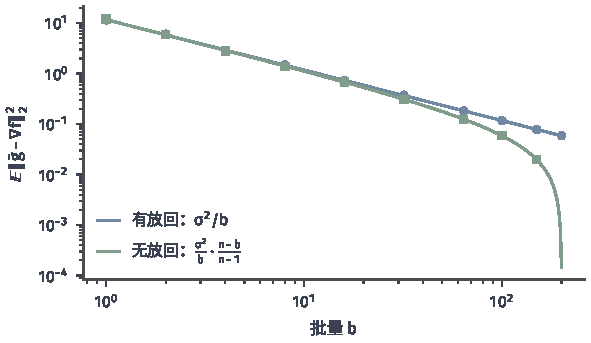
\includegraphics[width=100mm]{figures/03-optimization-evolution-and-signals/01-optimization/matplotlib/c6-minibatch-variance/figure.pdf}
  \caption{小批量读数的方差随批量$b$的变化。最小二乘$n=200$、$d=5$，在$\bm x=\bm0$处单项方差$\sigma^2\approx11.7$。实线为公式，圆点（有放回）与方块（无放回）为每个$b$各$4000$次抽样的经验值，双对数坐标。有放回时方差严格按$1/b$下降；无放回时在$b$接近$n$处迅速降到零，$b=n$时为零未画出。}
  \label{fig:opt-sto-minibatch}
\end{figure}

\paragraph{批量不能消除偏差}
批量平均只压低式~\eqref{eq:opt-sto-reading-split}中的噪声$\bm\xi$，对条件偏差$\bm\beta$毫无作用：$b$个有相同偏差的读数，平均后偏差不变。另外，批量为$b$的一步要读取$b$项，期望下降量却至多是精确梯度步的下降量。噪声已不是主要限制时，继续增大批量只是用$b$倍的读取换取几乎相同的一步，第~\ref{sec:opt-sto-cost}节会把这一点画成读取量随批量变化的曲线。

\paragraph{梯度累积}
批量受内存限制时，可以把它拆成若干微批量依次计算再合并，这称为\term{梯度累积}（gradient accumulation）。设一个批量$B$拆为$K$个不相交的微批量$B_1,\dots,B_K$，大小$n_j=|B_j|$，$N=\sum_jn_j$。要与一次读完$B$等价，必须满足下面算法中的约定。

\begin{algorithm}[梯度累积的一次更新]
\label{alg:opt-sto-accumulation}
\begin{algorithmic}[1]
\Require 当前参数$\bm x$（整个窗口内冻结），微批量$B_1,\dots,B_K$，步长$\eta$，确定的正则项$r$
\Ensure 新参数，以及只推进一次的调度时钟与优化器状态
\State $\bm s\gets\bm0$
\For{$j=1,\dots,K$}
  \State 在同一个$\bm x$处计算微批量平均$\bar{\bm g}_j=\frac1{n_j}\sum_{i\in B_j}\nabla\ell_i(\bm x)$
  \State $\bm s\gets\bm s+n_j\bar{\bm g}_j$ \Comment{按样本数加权}
\EndFor
\State $\bm g\gets\bm s/N+\nabla r(\bm x)$ \Comment{正则梯度只加一次}
\State $\bm x\gets\bm x-\eta\bm g$；调度时钟、动量与二阶统计各推进一次
\end{algorithmic}
\end{algorithm}

按样本数加权是必要的。若$n_1=2$、$n_2=1$，两组平均分别为$1$和$4$，正确的批量平均是$(2\cdot1+1\cdot4)/3=2$，直接平均两组得到$5/2$，相当于给第二组的样本加了双倍权重。等价性还要求窗口内每个样本被求值的函数和求值点与一次读完时相同：如果网络中有依赖批统计量的批归一化，或者随机失活在各微批量用了不同的随机状态，微批量上的函数就与大批量上的不同，结果不再一致。梯度累积减少的是同时驻留的中间结果，即存储；它仍要读取$N$项、做$K$次前向与反向计算，总读取量并不减少。

\subsection{SVRG}
\label{sec:opt-sto-svrg}

\paragraph{控制变量}
批量降噪需要每步多读，而且噪声只按比例缩小。另一种思路来自蒙特卡罗估计中的\term{控制变量}（control variate）：要估计$\mathbb E[Z]$，若有一个与$Z$高度相关、且期望$\mathbb E[Y]$已知的量$Y$，那么$Z-Y+\mathbb E[Y]$的期望仍是$\mathbb E[Z]$，方差却是$\mathbb E\lVert(Z-\mathbb EZ)-(Y-\mathbb EY)\rVert_2^2$，$Z$与$Y$越接近就越小。在有限和上，取$Z=\nabla f_i(\bm x)$，$Y=\nabla f_i(\tilde{\bm x})$为同一项在一个参考点$\tilde{\bm x}$处的梯度，它的期望$\nabla f(\tilde{\bm x})$只要在参考点算一次完整梯度就知道了。这就是\term{方差缩减}（variance reduction）方法SVRG的读数\scite{johnson2013accelerating}：
\begin{equation}
\label{eq:opt-sto-svrg}
  \bm v=\nabla f_i(\bm x)-\nabla f_i(\tilde{\bm x})+\tilde{\bm\mu},\qquad\tilde{\bm\mu}=\nabla f(\tilde{\bm x}).
\end{equation}
$i$均匀且与历史独立时，$\mathbb E_t[\bm v]=\nabla f(\bm x)-\nabla f(\tilde{\bm x})+\tilde{\bm\mu}=\nabla f(\bm x)$，读数条件无偏。

\begin{algorithm}[SVRG]
\label{alg:opt-sto-svrg}
\begin{algorithmic}[1]
\Require 初始快照$\tilde{\bm x}^{(0)}$，步长$\eta$，内循环长度$m$，外循环轮数$S$
\Ensure 最后的快照$\tilde{\bm x}^{(S)}$
\For{$s=0,1,\dots,S-1$}
  \State 计算完整梯度$\tilde{\bm\mu}=\nabla f(\tilde{\bm x}^{(s)})$ \Comment{读取$n$项}
  \State $\bm x^{(0)}\gets\tilde{\bm x}^{(s)}$
  \For{$k=0,1,\dots,m-1$}
    \State 均匀抽取$i$，$\bm v\gets\nabla f_i(\bm x^{(k)})-\nabla f_i(\tilde{\bm x}^{(s)})+\tilde{\bm\mu}$
    \State $\bm x^{(k+1)}\gets\bm x^{(k)}-\eta\bm v$
  \EndFor
  \State 均匀抽取$k\in\{0,\dots,m-1\}$，令$\tilde{\bm x}^{(s+1)}\gets\bm x^{(k)}$ \Comment{实践中常取$\bm x^{(m)}$}
\EndFor
\end{algorithmic}
\end{algorithm}

算法的状态是快照$\tilde{\bm x}$、快照处的完整梯度$\tilde{\bm\mu}$和当前点$\bm x$，存储$O(d)$。每步内循环要计算两个单项梯度；若改为保存全部$\nabla f_i(\tilde{\bm x})$，可省去一次计算，但存储变为$O(nd)$（对线性模型只需保存$n$个标量残差）。一个外循环的读取量是$n+2m$。

\paragraph{方差为何趋于零}
读数的噪声是$\bm v-\nabla f(\bm x)=[\nabla f_i(\bm x)-\nabla f_i(\tilde{\bm x})]-\mathbb E_t[\nabla f_i(\bm x)-\nabla f_i(\tilde{\bm x})]$。随机向量减去自身均值后，二阶矩不超过原二阶矩，所以若每项$L_{\max}$光滑，
\[
  \mathbb E_t\lVert\bm v-\nabla f(\bm x)\rVert_2^2\leq\frac1n\sum_{i=1}^n\lVert\nabla f_i(\bm x)-\nabla f_i(\tilde{\bm x})\rVert_2^2\leq L_{\max}^2\lVert\bm x-\tilde{\bm x}\rVert_2^2 .
\]
当前点与快照都接近最小点时，读数噪声随之趋于零，这是普通随机梯度做不到的：后者在最小点处的方差仍是$\sigma_\star^2$。三点例把这一点推到极端：$\nabla f_i(x)-\nabla f_i(\tilde x)=x-\tilde x$与$i$无关，于是$v=x-\tilde x+(\tilde x-2)=x-2$，每一步读数都精确等于真梯度。一般问题中各项曲率不同，噪声不为零，但会随$\bm x,\tilde{\bm x}\to\bm x^\star$而缩小。

\paragraph{强凸情形的线性收敛}
用引理~\ref{lem:opt-sto-cocoercive}可以把读数的二阶矩与目标差联系起来，再沿用距离递推。

\begin{lemma}[SVRG读数的二阶矩]
\label{lem:opt-sto-svrg-moment}
设每个$f_i$凸且$L_{\max}$光滑，$\bm x^\star$是$f$的最小点。则式~\eqref{eq:opt-sto-svrg}满足
\[
  \mathbb E_t\lVert\bm v\rVert_2^2\leq4L_{\max}\bigl(f(\bm x)-f^\star\bigr)+4L_{\max}\bigl(f(\tilde{\bm x})-f^\star\bigr).
\]
\end{lemma}

\begin{proof}
把$\bm v$写成$[\nabla f_i(\bm x)-\nabla f_i(\bm x^\star)]-[\nabla f_i(\tilde{\bm x})-\nabla f_i(\bm x^\star)-\nabla f(\tilde{\bm x})]$，用$\lVert\bm u-\bm w\rVert_2^2\leq2\lVert\bm u\rVert_2^2+2\lVert\bm w\rVert_2^2$。第一部分由引理~\ref{lem:opt-sto-cocoercive}及$\nabla f(\bm x^\star)=\bm0$，平均后不超过$2L_{\max}(f(\bm x)-f^\star)$。第二部分是随机向量$\nabla f_i(\tilde{\bm x})-\nabla f_i(\bm x^\star)$减去它的均值$\nabla f(\tilde{\bm x})$，二阶矩不超过未中心化的二阶矩，同理不超过$2L_{\max}(f(\tilde{\bm x})-f^\star)$。
\end{proof}

\begin{theorem}[SVRG的线性收敛]
\label{thm:opt-sto-svrg}
设每个$f_i$凸且$L_{\max}$光滑，$f$是$\mu$强凸的，$0<\eta<1/(4L_{\max})$，$m$满足
\[
  \alpha=\frac{1}{\mu\eta(1-2L_{\max}\eta)m}+\frac{2L_{\max}\eta}{1-2L_{\max}\eta}<1 .
\]
则算法~\ref{alg:opt-sto-svrg}满足$\mathbb Ef(\tilde{\bm x}^{(s+1)})-f^\star\leq\alpha\bigl(\mathbb Ef(\tilde{\bm x}^{(s)})-f^\star\bigr)$。
\end{theorem}

\begin{proof}
固定一个外循环，记$\tilde{\bm x}=\tilde{\bm x}^{(s)}$。与引理~\ref{lem:opt-sto-distance}的证明相同地展开$\lVert\bm x^{(k+1)}-\bm x^\star\rVert_2^2$，内积项用凸性$\langle\nabla f(\bm x),\bm x-\bm x^\star\rangle\geq f(\bm x)-f^\star$，平方项用引理~\ref{lem:opt-sto-svrg-moment}，得到
\[
  \begin{aligned}
    \mathbb E_k\lVert\bm x^{(k+1)}-\bm x^\star\rVert_2^2
    &\leq\lVert\bm x^{(k)}-\bm x^\star\rVert_2^2-2\eta(1-2L_{\max}\eta)\bigl(f(\bm x^{(k)})-f^\star\bigr)\\
    &\quad+4L_{\max}\eta^2\bigl(f(\tilde{\bm x})-f^\star\bigr).
  \end{aligned}
\]
对$k=0,\dots,m-1$取期望求和，距离项相消，再用$\bm x^{(0)}=\tilde{\bm x}$与强凸性$\lVert\tilde{\bm x}-\bm x^\star\rVert_2^2\leq\tfrac2\mu(f(\tilde{\bm x})-f^\star)$：
\[
  2\eta(1-2L_{\max}\eta)\sum_{k=0}^{m-1}\mathbb E\bigl(f(\bm x^{(k)})-f^\star\bigr)\leq\Bigl(\frac2\mu+4L_{\max}\eta^2m\Bigr)\bigl(f(\tilde{\bm x})-f^\star\bigr).
\]
新快照在$\bm x^{(0)},\dots,\bm x^{(m-1)}$中均匀选取，左边求和恰为$m\,\mathbb E(f(\tilde{\bm x}^{(s+1)})-f^\star)$的$2\eta(1-2L_{\max}\eta)$倍。两边相除即得$\alpha$。
\end{proof}

以$\kappa_{\max}=L_{\max}/\mu$计，取$\eta=1/(10L_{\max})$，$1-2L_{\max}\eta=0.8$，第二项为$0.25$；取$m=50\kappa_{\max}$，第一项为$1/(\tfrac1{10\kappa_{\max}}\cdot0.8\cdot50\kappa_{\max})=0.25$，于是$\alpha=1/2$。每个外循环把目标差减半，读取量为$n+2m=n+100\kappa_{\max}$，达到精度$\varepsilon$总共需要$O\bigl((n+\kappa_{\max})\log(1/\varepsilon)\bigr)$次读取。作为对照，梯度下降需要$O(n\kappa\log(1/\varepsilon))$次读取，普通随机梯度由定理~\ref{thm:opt-sto-decreasing}需要$O(\sigma_\star^2/(\mu^2\varepsilon))$量级的迭代：前者每步太贵，后者对$\varepsilon$不是对数依赖。定理的常数偏保守，实践中常用更大的步长，取最后一点作为新快照，并把$m$取为$n$的若干倍；这些改动需要另行核验。

\subsection{SAGA}
\label{sec:opt-sto-saga}

\paragraph{用梯度记忆代替快照}
SVRG的参考点每隔$m$步才更新一次，而且每次更新要读全部数据。SAGA改为给每一项各存一份“最近一次读到的梯度”$\bm\phi_i$，并维护它们的平均$\bar{\bm\phi}=\frac1n\sum_i\bm\phi_i$\scite{defazio2014saga}。抽到第$j$项时，用新旧读数之差纠偏：
\begin{equation}
\label{eq:opt-sto-saga}
  \bm v=\nabla f_j(\bm x)-\bm\phi_j+\bar{\bm\phi},
\end{equation}
然后用$\bm v$更新参数，再把$\bm\phi_j$替换为$\nabla f_j(\bm x)$、把$\bar{\bm\phi}$加上$(\nabla f_j(\bm x)-\bm\phi_j)/n$。

\begin{algorithm}[SAGA]
\label{alg:opt-sto-saga}
\begin{algorithmic}[1]
\Require 初值$\bm x^{(0)}$，步长$\eta$，轮数$T$
\Ensure 最后一点$\bm x^{(T)}$
\State 对每个$i$置$\bm\phi_i\gets\nabla f_i(\bm x^{(0)})$，$\bar{\bm\phi}\gets\frac1n\sum_i\bm\phi_i$ \Comment{读取$n$项}
\For{$t=0,1,\dots,T-1$}
  \State 均匀抽取$j$，计算$\bm u\gets\nabla f_j(\bm x^{(t)})$
  \State $\bm v\gets\bm u-\bm\phi_j+\bar{\bm\phi}$ \Comment{用更新前的平均}
  \State $\bm x^{(t+1)}\gets\bm x^{(t)}-\eta\bm v$
  \State $\bar{\bm\phi}\gets\bar{\bm\phi}+(\bm u-\bm\phi_j)/n$，$\bm\phi_j\gets\bm u$
\EndFor
\end{algorithmic}
\end{algorithm}

\paragraph{哪一个平均保证无偏}
算法中构造$\bm v$用的是\emph{更新前}的$\bar{\bm\phi}$。此时表$\bm\phi_1,\dots,\bm\phi_n$由历史决定，$\mathbb E_t[\nabla f_j(\bm x)-\bm\phi_j]=\nabla f(\bm x)-\bar{\bm\phi}$，加上$\bar{\bm\phi}$后正好是$\nabla f(\bm x)$。若先更新平均再构造方向，读数变为$\bm v'=\bm v+(\nabla f_j(\bm x)-\bm\phi_j)/n$，条件期望多出$(\nabla f(\bm x)-\bar{\bm\phi})/n$，只要表还没有追上当前梯度就有偏。条件无偏来自“新读数减去同一项的旧读数”，旧读数的平均必须是构造方向那一刻的已知量。

三点例同样能看清记忆的作用。设第$i$项上次被读取时参数为$x_{k_i}$，则$\phi_i=x_{k_i}-c_i$，代入式~\eqref{eq:opt-sto-saga}得$v=x-x_{k_j}+\frac13\sum_ix_{k_i}-2$。数据值$c_i$完全消去，噪声只来自各项记录的“年龄”不同。表刚初始化时所有$x_{k_i}$相同，$v$恰为真梯度；随着迭代收敛，各次记录的参数彼此接近，噪声也趋于零。

\paragraph{误差的两个来源与代价}
分析SAGA时，误差不只在参数上，还在表里：表中的旧梯度离$\nabla f_i(\bm x^\star)$越远，读数噪声越大。因此收敛证明使用同时包含两部分的势函数，形如$\lVert\bm x-\bm x^\star\rVert_2^2+c\cdot\frac1n\sum_i\lVert\bm\phi_i-\nabla f_i(\bm x^\star)\rVert_2^2$。在每项凸且$L_{\max}$光滑、$f$为$\mu$强凸的条件下，取步长$1/(3L_{\max})$时，期望距离按每步$1-\min\{1/(4n),\mu/(3L_{\max})\}$的比率线性收敛\scite{defazio2014saga}。$n$大时比率由$1/(4n)$决定，即大约每遍历一次数据误差缩小一个常数因子，与SVRG的总读取量同阶。

图~\ref{fig:opt-sto-variance-reduction}在$n=200$、$d=10$的岭逻辑回归上比较五种方法，横轴统一为读取量。常数步长的随机梯度很快停在约$10^{-2}$的平台，递减步长继续缓慢下降；梯度下降每步读$n$项，在$30$遍数据内只走$30$步。SVRG与SAGA则保持线性收敛，(b)显示其原因：普通随机梯度的方向方差始终约为$1$，SVRG的方差在每次快照时归零、随后回升，整体逐轮下降，SAGA的方差随表的更新稳步下降。

\begin{figure*}[!htbp]
  \centering
  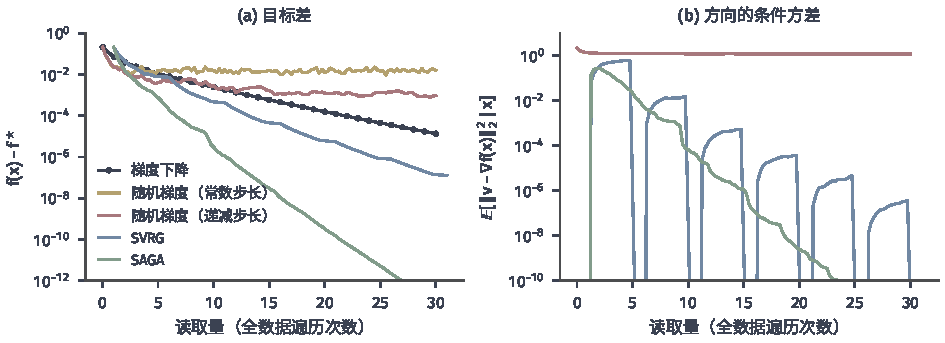
\includegraphics[width=160mm]{figures/03-optimization-evolution-and-signals/01-optimization/matplotlib/c6-variance-reduction/figure.pdf}
  \caption{方差缩减方法与随机梯度的比较。岭逻辑回归，$n=200$，$d=10$，$\lambda=0.05$，$L\approx0.71$，$L_{\max}\approx10.0$，$8$个随机种子平均。横轴为读取量除以$n$；梯度下降每步读$n$项，SVRG每个外循环读$n+2m$项（$m=2n$），SAGA初始化读$n$项、此后每步读$1$项。步长：梯度下降$1/L$，随机梯度$1/(2L_{\max})$（递减版本再除以$1+t/(2n)$），SVRG与SAGA均为实验取值$1/(3L_{\max})$，比定理~\ref{thm:opt-sto-svrg}所需的保守常数大。(a) 目标差；(b) 当前点处方向读数的条件方差，由全部$n$项精确计算。}
  \label{fig:opt-sto-variance-reduction}
\end{figure*}

代价方面，SAGA每步只读一项、不需要周期性的全数据遍历，但要存储$n$个梯度，一般为$O(nd)$；对线性模型$\nabla f_i(\bm x)=\ell_i'(\bm a_i^\top\bm x)\bm a_i+\lambda\bm x$，只需存$n$个标量$\ell_i'$。更根本的限制是适用范围：SVRG和SAGA都要求能反复访问同一项，这是有限和的结构。对只能不断获得新样本的期望目标~\eqref{eq:opt-sto-expectation}，每个样本只见一次，既没有可复用的旧读数，也无法计算快照处的完整梯度，两种方法不能原样使用。
